\documentclass[../main.tex]{subfiles}
\begin{document}

\section[Уравнение теплопроводности в \texorpdfstring{$\R^1$}{R}]{Формула Пуассона решения задачи Коши для однородного уравнения теплопроводности в $\R^1$. Фундаментальное решение. Существование классического решения задачи Коши при непрерывной ограниченной начальной функции.}

$$\text{Задача: \ }
\begin{cases}
	u_t - a^2u_{xx} = 0, &x \in \R,\ t > 0 \\
	u\bigr|_{t = 0} = u_0(x), &x \in \R
\end{cases} $$

\Subsection{Наводящие соображения}

На \href{https://drive.google.com/file/d/15t8c9cRmu38MEu2vC06M9binZ6IPNt1k/view?usp=sharing"}{консультации} 2021 года лектор сказал, что эту часть можно не учить. Поэтому можете сразу перейти к \hyperref[sec:FormalProof]{формальному доказательству формулы Пуассона.}
\vspace{0.7em}
% Исходная ссылка Зубова https://drive.google.com/file/d/138e2xKJtS3EVTUY8himJiMg2n9gQu96B/view 

Итак, пусть для начала:
\begin{equation*}
u_0(x) = \begin{cases} 
	1, &x \geq 0, \\
	0, &x < 0 
\end{cases} 
\end{equation*}
Сделаем замену: 
\begin{equation*}
\begin{cases}
	\tau = \alpha t, &\alpha > 0, \\
	\xi = \beta x, &\beta > 0.
\end{cases}
\end{equation*}
Пусть $u(t, x)$ - решение задачи. \ Введём $v(\tau, \xi) = u\left(\dfrac{\tau}{\alpha},\ \dfrac{\xi}{\beta}\right)$. \ Тогда
\begin{enumerate}
	\vspace{-0.7em} % Мне показалось, что отступ между текстом и первым элементом слишком большой. Я мог бы использовать \begin{enumerate}[topsep = 0em], но тогда отступ после последнего элемента тоже бы уменьшился
	\item \qquad $v\bigr|_{\tau=0} = \begin{cases} \begin{aligned}
		1, \quad && \frac{\xi}{\beta} \geq 0 &&\Leftrightarrow && \xi \geq 0 \\
		0, \quad && \frac{\xi}{\beta} < 0 && \Leftrightarrow && \xi < 0
	\end{aligned}\end{cases}$

	\item \qquad $v_\tau = \dfrac{1}{\alpha}u_t, \quad v_\xi = \dfrac{1}{\beta}\, u_x, \quad v_{\xi \xi} = \dfrac{1}{\beta^2}\, u_{xx} \qquad\Rightarrow\qquad \alpha v_{\tau} = a^2 \beta^2 v_{\xi \xi}$
\end{enumerate}

Функция $v$ в общем случае будет решением другой задачи Коши, но при $\alpha = \beta^2$ --- той же самой задачи Коши. Значит, решение не единственно: если $u(t,x)$ --- решение, то $\,\forall\, \beta > 0$ функция $v(t,x) = u\left(\dfrac{t}{\beta^2},\ \dfrac{x}{\beta}\right)$ --- тоже решение.

\begin{definition} 
Множество преобразований $\{u_{\alpha}\}_{\alpha \in \mathcal{D}}$ --- \emph{однопараметрическая группа преобразований,} если:
\begin{itemize}
	\item Это множество замкнуто относительно операции композиции:
	$$\forall\, \alpha, \beta \in \mathcal{D} \quad \exists!\,\gamma \in \mathcal{D}\colon \quad u_\alpha \circ u_\beta = u_\gamma$$
	
	\item Оно содержит нейтральный элемент --- тождественное преобразование:
	$$\exists!\, o \in \mathcal{D} \quad \bigl(\forall\, \alpha \in \mathcal{D} \quad u_o \circ u_\alpha = u_\alpha \circ u_o = u_\alpha \bigr)$$
	
	\item У каждого элемента есть обратный, и их композиция в любом порядке даёт тождественное преобразование.
\end{itemize}
\end{definition}
	
\begin{definition}
	Функция $I(x)$ --- \textit{инвариант однопараметрической группы преобразовний}, если $\Forall \alpha \in \mathcal{D} \quad I(x) \equiv I(u_{\alpha}(x))$
	\end{definition}
	\begin{definition}
	Говорят, что \textit{уравнение допускает однопараметрическую группу преобразований}, если все преобразования группы переводят решения этого уравнения в решения.\footnote{В прошлых версиях файла определение гласило, что уравнение допускает группу преобразований, если оно инвариантно относительно всех преобразований группы. Но непонятно, что подразумевается под инвариантностью \emph{уравнения}. Новое определение же опирается на инвариантность \emph{функций}. Оно взято с \href{https://matem.anrb.ru/bsuconf/2012/adlerv7.pdf}{этого сайта.}}
\end{definition}

\begin{definition}
Решение уравнения называется \textit{автомодельным}, если оно зависит только от инвариантов некоторой допустимой группы преобразований.
\end{definition}
\begin{example}
Множество преобразований
\begin{equation*}
\begin{cases}
	\tau = \beta^2 t, \\
	\xi = \beta x
\end{cases}
\end{equation*}
есть однопарметрическая группа преобразований, $z = \dfrac{x}{\sqrt{t}} $ --- инвариант группы.
\end{example}
Найдём автомодельное решение $u(t, x) = f\brk*{\dfrac{x}{\sqrt{t}}} = f(z)$. \\
В этом случае:
\begin{equation*}
	u_t = f'\brk*{\dfrac{x}{\sqrt{t}}} \cdot \brk*{\frac{-x}{2t^{3/2}}} 
	\qquad u_x = f'\brk*{\frac{x}{\sqrt{t}}} \cdot \frac{1}{\sqrt{t}} 
	\qquad u_{xx} = f''\brk*{\frac{x}{\sqrt{t}}} \cdot \frac{1}{t}
\end{equation*}

Подставляем в уравнение:
\vspace{-0.7em}
\begin{align*}
	&-\frac{x}{2t\sqrt{t}} f'(z) = a^2 f''(z) \cdot \frac{1}{t}\\[0.3em]
	&\frac{f''(z)}{f'(z)} = - \frac{1}{a^2} \frac{x}{2\sqrt t} = -\frac{1}{2 a^2} z\\[0.2em]
	&\ln|f'(z)| = -\frac{z^2}{4a^2} + \tilde{C}_1
\end{align*}
Получили, что \ $f(z) = C_1 \displaystyle \int\limits_{-\infty}^z \expT{-\frac{\eta^2}{4a^2}}\, d\eta + C_2$
\paragraph{Задача была следующей:} бесконечный стержень разделён на две половины, начальные температуры половин $T_0 = 0$ и $T_1 = 1$. Из физических соображений:
\begin{flalign*}
	& \lim\limits_{z \to - \infty} f(z) = 0 \quad \Rightarrow \quad C_2 = 0 & \\
	& \lim\limits_{z \to + \infty} f(z) = 1 \quad \Rightarrow \quad \int\limits_{-\infty}^{+\infty} \expT{-\frac{\eta^2}{4a^2}}\, d \eta = C_1^{-1} = 2a \underbrace{\int\limits_{-\infty}^{+\infty} \expT{-\frac{\eta^2}{4a^2}}\, d \frac{\eta}{2a}}_{\sqrt{\pi}} \quad\ \Rightarrow \quad\ C_1 = \frac{1}{\sqrt{4 \pi a^2}} &
\end{flalign*}
Окончательно:
\begin{equation*}
	f(z) = \frac{1}{\sqrt{4 \pi a^2}}\int\limits_{-\infty}^{z} \expT{-\frac{\eta^2}{4a^2}}\, d \eta = \frac{2a}{\sqrt{4 \pi a^2}} \int\limits_{-\infty}^{z/2a}e^{-\mu^2}\, d \mu = \frac{1}{\sqrt{\pi}} \int\limits_{-\infty}^{z/2a}e^{-\mu^2}\, d \mu 
\end{equation*}
Введём \textbf{интеграл ошибок}:
\begin{equation*}
	\erf(z) = \frac{2}{\sqrt{\pi}} \int\limits_{0}^{z}e^{-\xi^2}\, d \xi\, , \qquad \erf(\pm \infty) = \pm 1,\; \; \erf(0) = 0
\end{equation*}
Тогда:
\begin{equation*}
	u(t, x) = f\brk*{\frac{x}{\sqrt{t}}} = \frac{1}{\sqrt{\pi}} \int\limits_{-\infty}^{\frac{x}{\sqrt{4 t a^2}}} e^{-\mu^2}\, d \mu = \frac{1}{2}\brk[s]*{1 + \erf\brk*{\frac{x}{\sqrt{4 a^2 t}}}}
\end{equation*}
\begin{enumerate}
\item Мы рассмотрели модельную задачу
\begin{center}
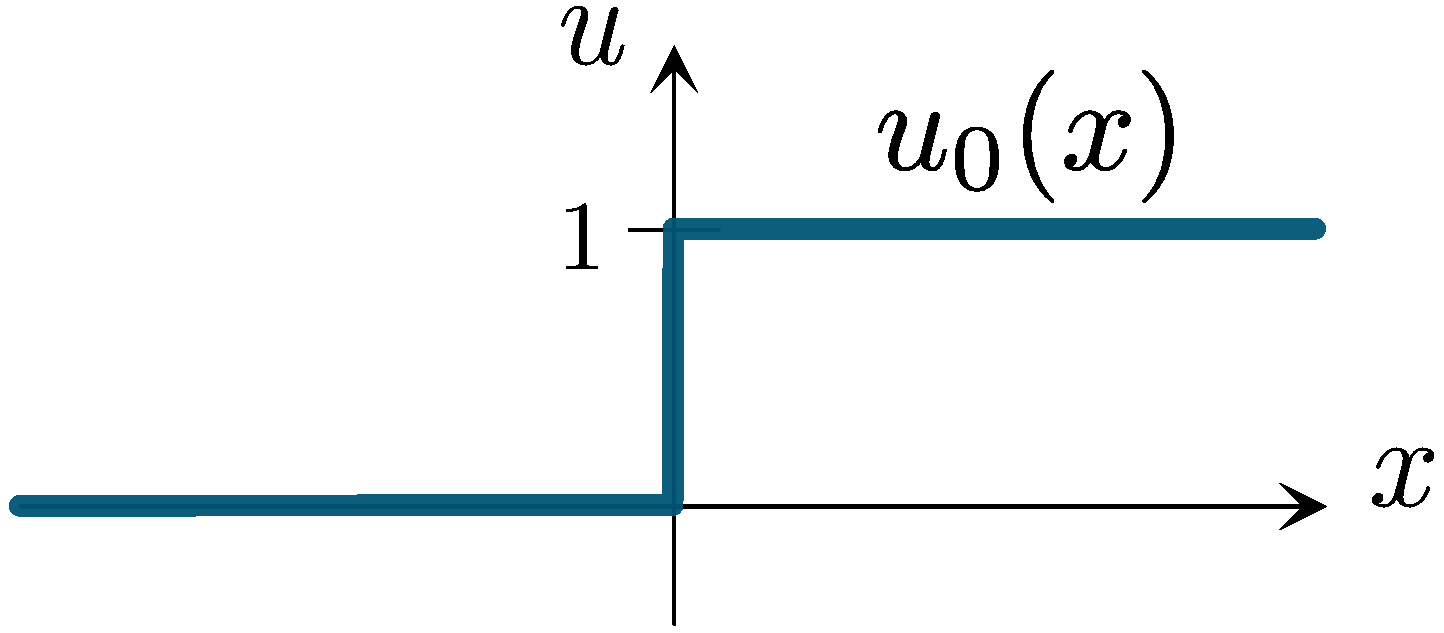
\includegraphics[height=0.11\textwidth]{./pic 9_1.pdf}
\end{center}
\item Увеличим ступеньку в $u_*$ раз и сдвинем
$$u(t,x) = \frac{u_*}{2}\brk[s]*{1+\erf \brk*{\frac{x-x_0}{\sqrt{4a^2t}}}}$$
\item Можем получить и решение для ступеньки конечной ширины:
$$u(t,x) = \frac{u_*}{2}\brk[s]*{\erf \brk*{\frac{x-x_1}{\sqrt{4a^2t}}}-\erf \brk*{\frac{x-x_2}{\sqrt{4a^2t}}}}$$
\item Для системы из $N$ интервалов имеем:
\begin{center}
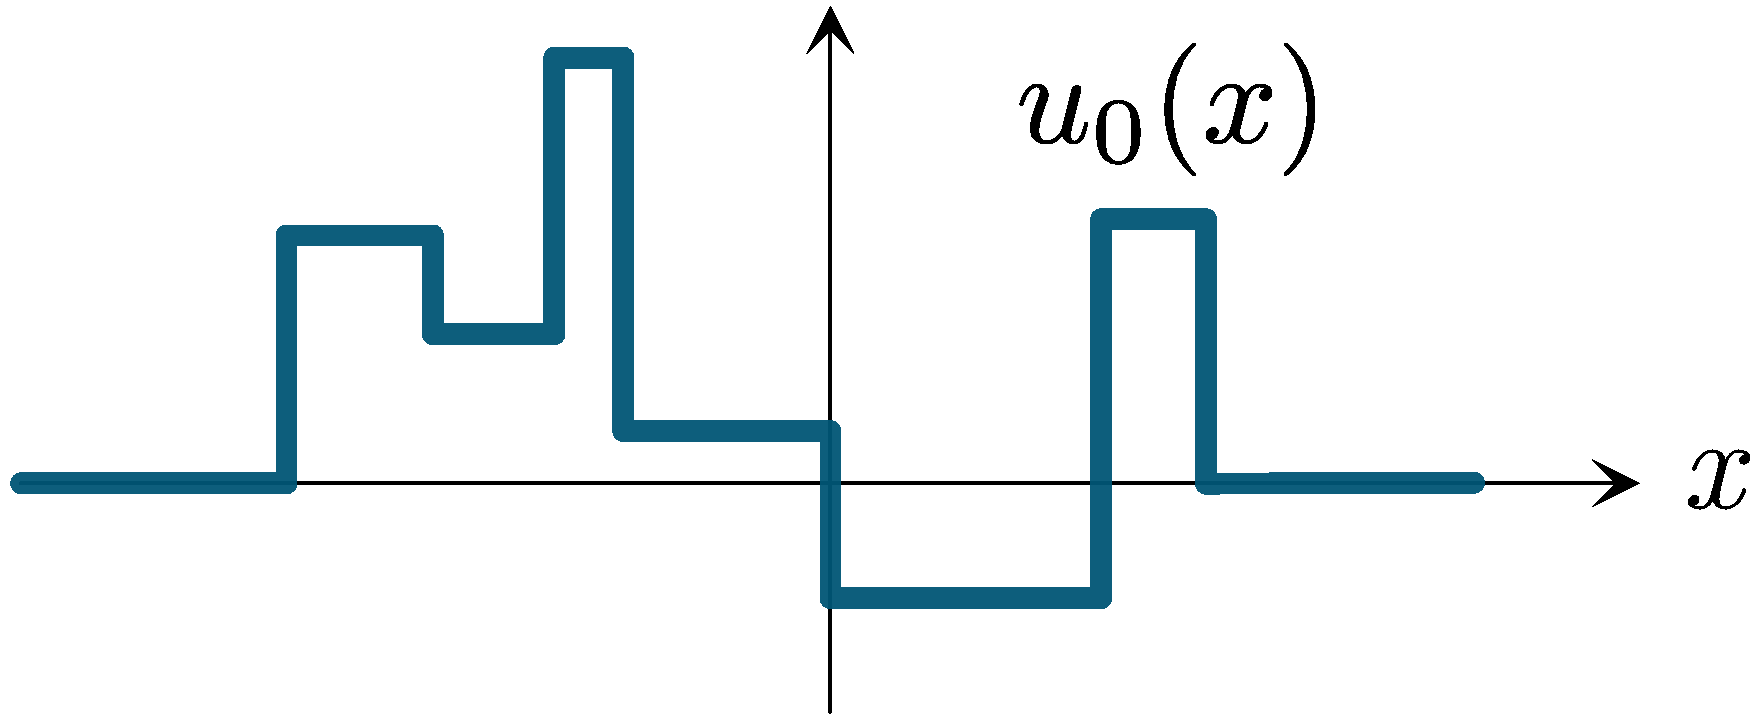
\includegraphics[height=0.125\textwidth]{./pic 9_2.pdf}
\end{center}
$$u(t,x) = \sum_{k=1}^{N}\frac{u_{*k}}{2}\brk[s]*{\erf \brk*{\frac{x-x_{1k}}{\sqrt{4a^2t}}}-\erf \brk*{\frac{x-x_{2k}}{\sqrt{4a^2t}}}}$$

Последнее можно переписать в следующем виде:
$$u(t,x) = \sum_{k=1}^{N}\brk[s]*{\frac{\brk[c]*{-\frac{1}{2}\erf \brk*{\frac{x-x_{2k}}{\sqrt{4a^2t}}}}-\brk[c]*{-\frac{1}{2}\erf \brk*{\frac{x-x_{1k}}{\sqrt{4a^2t}}}}}{x_{2k}-x_{1k}}}u_{*k} \cdot (x_{2k} - x_{1k})$$
\item Окончательно, пусть $u_0(x)$ финитна, непрерывна, ограничена. Разбиваем ее носитель $\supp u_0(x)$ на отрезки, аппроксимируем кусочно постоянной. Для приближенных решений справедливо:
\begin{align*}
u(t,x) &= \brk[s]*{
		\Psi (t,x, \xi) = -\frac{1}{2} \erf\brk*{\frac{x - \xi}{\sqrt{4a^2t}}}
		,\quad \xi_k = \frac{x_{2k} - x_{1k}}{2}
	} = \\[0.7em] 
& = \sum_{k=1}^N \frac{
		\Psi(t,x,x_{2k})-\Psi(t,x,x_{1k})
	}{x_{2k}-x_{1k}} 
	\cdot u_{*k} \cdot
	(x_{2k} - x_{1k}) \approx\\[0.7em]
& \approx \sum_{k=1}^N \eval*{ \pd{\Psi}{\xi} }_{ \xi = \xi_k } 
	u_0(\xi_k) (x_{2k} - x_{1k}) 
	= \brk[s]*{
		\pd{\Psi}{\xi} = \frac{1}{\sqrt{4 \pi a^2 t}}\, \expT{-\frac{(x-\xi)^2}{4a^2t}}
		} = \\[0.7em]
&= \sum_{k=1}^N \frac{1}{\sqrt{4 \pi a^2 t}} \eval*{
		\expT{-\frac{(x-\xi)^2}{4a^2t}}
	}_{\xi = \xi_k}
	u_0(\xi_k) (x_{2k} - x_{1k}) \text{ \ --- \ Интегральная сумма Римана}
\end{align*}

Предположение: решение будет 
$$
u(t,x) = \frac{1}{\sqrt{4\pi a^2 t}} \int_{-\infty}^{\infty} \expT{-\frac{(x-\xi)^2}{4a^2t}} u_0(\xi)\, d\xi 
\text{ \ --- \ Формула Пуассона} $$
Функция \imaginarySubsection{Фундаментальное решение}
$$\mathcal{E}(t,x) =  \frac{1}{\sqrt{4\pi a^2 t}} \expT{-\frac{x^2}{4a^2 t}} \textbf{\, ---\, фундаментальное решение (или функция источника)}$$
\end{enumerate}

\Subsection[Формула Пуассона]{Строгое доказательство} \label{sec:FormalProof} \imaginarySubsection{Свойства решения}


\begin{theorem}
Пусть $u_0\in C(\R^1),\;\; \abs*{u_0(x)}\leq M_0 \;\;\forall\, x\in \R^1.$ \ Тогда функция 
$$u(t,x) = \frac{1}{\sqrt{4\pi a^2 t}} \int_{-\infty}^{\infty} \expT{-\frac{(x - y)^2}{4a^2t}} u_0(y) dy$$
\begin{enumerate}

\item Принадлежит классу $C^{\infty}\, (t>0,\ x\in\R^1) \ \cap\ C(t \geq 0,\ x\in\R^1)$

\item Является классическим решением задачи Коши
\begin{equation*}
\begin{cases}
	u_t - a^2u_{xx} = 0, &x \in \R,\ t > 0 \\
	u\bigr|_{t = 0} = u_0(x), &x \in \R
\end{cases}
\end{equation*}

\item $\abs*{u(t,x)}\leq M \;\; \Forall t \geq 0, \Forall x\in\R^1$
\end{enumerate}
\end{theorem}

\newpage

\begin{proof}
\hfill
\begin{enumerate}
\item 
В исходном интеграле для $u(t,x)$ сделаем такую замену:
\[
\frac{y-x}{\sqrt{4 a^2 t}}=\eta, 
\quad  y = x + \sqrt{4 a^2 t}\,\eta,
\quad dy = \sqrt{4 a^2 t}\, d\eta
\]
Тогда получим
\begin{multline*}
u(t,x)=\frac{1}{\sqrt{\pi}}\int_{-\infty}^{\infty}e^{-\eta^2} u_0(x+\sqrt{4 a^2 t}\, \eta)\: d\eta \\
u_0(x+\sqrt{4 a^2 t}\,\eta) 
\;\ \in \;\ C(t \geq 0,\ x \in \R^1,\ \eta \in \R^1) \hspace{8.5em}
\end{multline*}
Оценим $\abs*{e^{-\eta^2} u_0(x+\sqrt{4 a^2 t}\, \eta)}\leq M_0e^{-\eta^2}$, причем $\displaystyle\int_{-\infty}^{\infty}M_0e^{-\eta^2}d\eta$ \ сходится $\ \Rightarrow\ $ исходный интеграл сходится равномерно, а значит лежит в $C(t\geq 0,\ x\in\R^1)$. Отсюда следует третье утверждение теоремы.

\item Возьмем 
\begin{equation}
u_x(t, x)\sim \int_{-\infty}^{\infty}\frac{1}{4a^3\sqrt{\pi}t^{3/2}}\expT{-\frac{(x-y)^2}{4a^2t}} (y-x)u_0(y)\, dy
\label{eq:9:u_x}
\end{equation}
Выражение под интегралом лежит в $C(t > 0,\;\: x, y \in \R^1)$. 

Пусть $x \in [-A, A]$. Покажем равномерную сходимость интеграла серией оценок:

\begin{enumerate}

	\item При $|y|>A \colon\ $

	$(y-x)^2 \geq (|y|-A)^2
	=y^2 + A^2 - 2\dfrac{|y|}{\sqrt{2}}\brk*{\sqrt{2}A}.$

	Поскольку $2ab \leq a^2 + b^2$,

	$(y-x)^2 \geq y^2+A^2-\dfrac{y^2}{2}-2A^2=\dfrac{y^2}{2}-A^2$
	\vspace{0.3em}

	\item При $\abs*{y}\leq A \colon\ (x-y)^2 > 0$

	\item При 
	$ \forall\, y \in \R\colon\ (x-y)^2 \geq \phi_A(y) 
	= \begin{cases}
		\dfrac{y^2}{2}-A^2,\   &\abs*{y}\geq A \\
		0,\                    &\abs*{y}  <  A
	\end{cases}
	$

	\item Кроме того, $\abs*{y-x}\leq \abs*{y}+A$.
	\end{enumerate}

Получили следующую оценку (при $|x| < A$):
\[
\abs*{\frac{1}{4a^3\sqrt{\pi}t^{3/2}}\expT{-\frac{(x-y)^2}{4a^2t}} (y-x)u_0(y)}\leq \frac{M_0}{4a^3\sqrt{\pi}t^{3/2}}(\abs*{y}+A)\expT{-\frac{\phi_A(y)}{4a^2t}}
\]
Если $t \in [t_1, t_2] \subset (0, +\infty)$, то это можно ограничить выражением $C \cdot (|y| + A) \cdot \expT{\frac{\phi_A(y)}{B}},$ интеграл от которого сходится, поэтому исходный интеграл сходится равномерно.

Равномерная сходимость (по двум параметрам сразу) есть в любом прямоугольнике 
$$Q = \Bigl\{ |x| < A, \;\ t \in [t_1, t_2] \Bigr\}$$
Беря в качестве $Q$ все возможные такие прямоугольники, получим, что производная $u_x$ на всём множестве $\bigl\{ t > 0,\ x \in \R^1 \bigr\}$ существует, непрерывна и равна интегралу \eqref{eq:9:u_x}.

Аналогично будет для любой другой производной (будет асимптотика $\abs*{P_n(y)}e^{-\alpha y^2}$).
\item%
\[
\begin{split}
&\mathcal{E} (t, x-y)=\frac{1}{\sqrt{4\pi a^2t}}\,\expT{-\frac{(x-y)^2}{4a^2t}} \\[7pt]
& \mathcal{E}_x(t,x-y) = -\frac{(x-y)}{2a^2 t}\cdot \mathcal E(t,x-y) \\[7pt]
& \mathcal{E}_{xx}(t,x-y) = \brk*{-\frac{1}{2a^2 t} + \frac{(x-y)^2}{4a^4 t^2}} \mathcal E(t,x-y) \\[7pt]
& \mathcal{E}_t(t,x-y) = \brk*{-\frac{1}{2}\frac{1}{t} + \frac{(x-y)^2}{4a^2}\frac{1}{t^2}} \mathcal E(t,x-y) \\[7pt]
\end{split}
\]
Тогда 
\[
u_t-a^2u_{xx}=\int\limits_{-\infty}^{+\infty}\cancelto{0}{\left[\mathcal{E}_t(t, x-y)-a^2\mathcal{E}_{xx}(t, x-y) \right]}u_0(y)dy=0.
\]
Начальное условие (используя самое начало выкладок)
\[
\eval{u}_{t=0}=\frac{1}{\sqrt{\pi}}\int\limits_{-\infty}^{+\infty}e^{-\eta^2}u_0(x)d\eta = u_0(x)
\]
\end{enumerate}
Теорема доказана.
\end{proof}




\end{document}